% Chapter 5 -- structure from table of content.md; impersonal academic style

\reportchapter{5}{System Evaluation and Performance Analysis}{}

\section{Introduction}

This chapter evaluates the platform introduced in Chapters~1--4 using a
curated benchmark designed for political and geopolitical question answering.
The objective is to measure the end-to-end behavior of the Graph-RAG
architecture, including evidence retrieval, graph-supported reasoning,
citation-grounded answer generation, ingestion-time knowledge extraction, and
the effect of alternative reasoning modes. The chapter first defines the
benchmark and experimental protocol, then presents the evaluation metrics and
quantitative results, before examining DSPy-based extraction optimization,
requirements validation, and threats to validity.

\section{Evaluation Methodology}

Evaluation was designed to assess the system as a complete platform rather
than as a collection of isolated components. Each benchmark question is
processed under realistic operating conditions, and the generated answer,
retrieved passages, and supporting graph facts are compared with a reference
answer. This end-to-end protocol ensures that the reported results reflect the
combined behavior of ingestion, indexing, retrieval, reasoning, and answer
generation.

\textbf{Benchmark construction and question categories.} A curated benchmark
of \textbf{150 questions} was created to represent the principal analytical
tasks encountered in the selected political and geopolitical domain. The
questions are grouped into four categories: \textbf{factual} questions address
direct entities, events, and dates; \textbf{relational} questions examine
connections between actors or institutions; \textbf{temporal} questions focus
on chronology and time-sensitive claims; and \textbf{comparative} questions
require synthesis across several sources, actors, or positions. Each
evaluation sample contains a question, a reference answer, and the evidence
required to assess retrieval and generation quality. This composition covers
both direct retrieval and graph-dependent reasoning as described in
Chapter~3.

\begin{table}[H]
\centering
\small
\setlength{\tabcolsep}{5pt}
\renewcommand{\arraystretch}{1.25}
\begin{tabularx}{\textwidth}{@{}>{\bfseries\raggedright\arraybackslash}p{2.5cm}>{\centering\arraybackslash}p{1.8cm}X@{}}
\toprule
\rowcolor{lightblue}
Category & Questions & Evaluation focus \\
\midrule
Factual & 40 & Direct retrieval of actors, institutions, dates, and events. \\
Relational & 40 & Connections requiring entity resolution or graph traversal. \\
Temporal & 35 & Chronology, validity intervals, and time-sensitive claims. \\
Comparative & 35 & Multi-source comparison of actors, policies, or positions. \\
\midrule
Total & 150 & Balanced coverage of direct and multi-hop political analysis. \\
\bottomrule
\end{tabularx}
\caption{Distribution of the 150-question benchmark.}
\label{tab:benchmark-distribution}
\end{table}

\textbf{Evaluation pipeline.} Each sample is evaluated using one of three
reasoning modes: standard RAG, chain-of-thought (CoT), or reflexive reasoning.
For every execution, the evaluation process records the generated answer,
cited sources, supporting graph facts, response time, and execution status.
The answer and retrieved evidence are subsequently assessed using lexical,
semantic, and RAGAS-based measures. This procedure supports both per-question
analysis and aggregate comparison across reasoning modes without allowing
unsuccessful executions to distort the reported averages.

\begin{figure}[H]
    \centering
    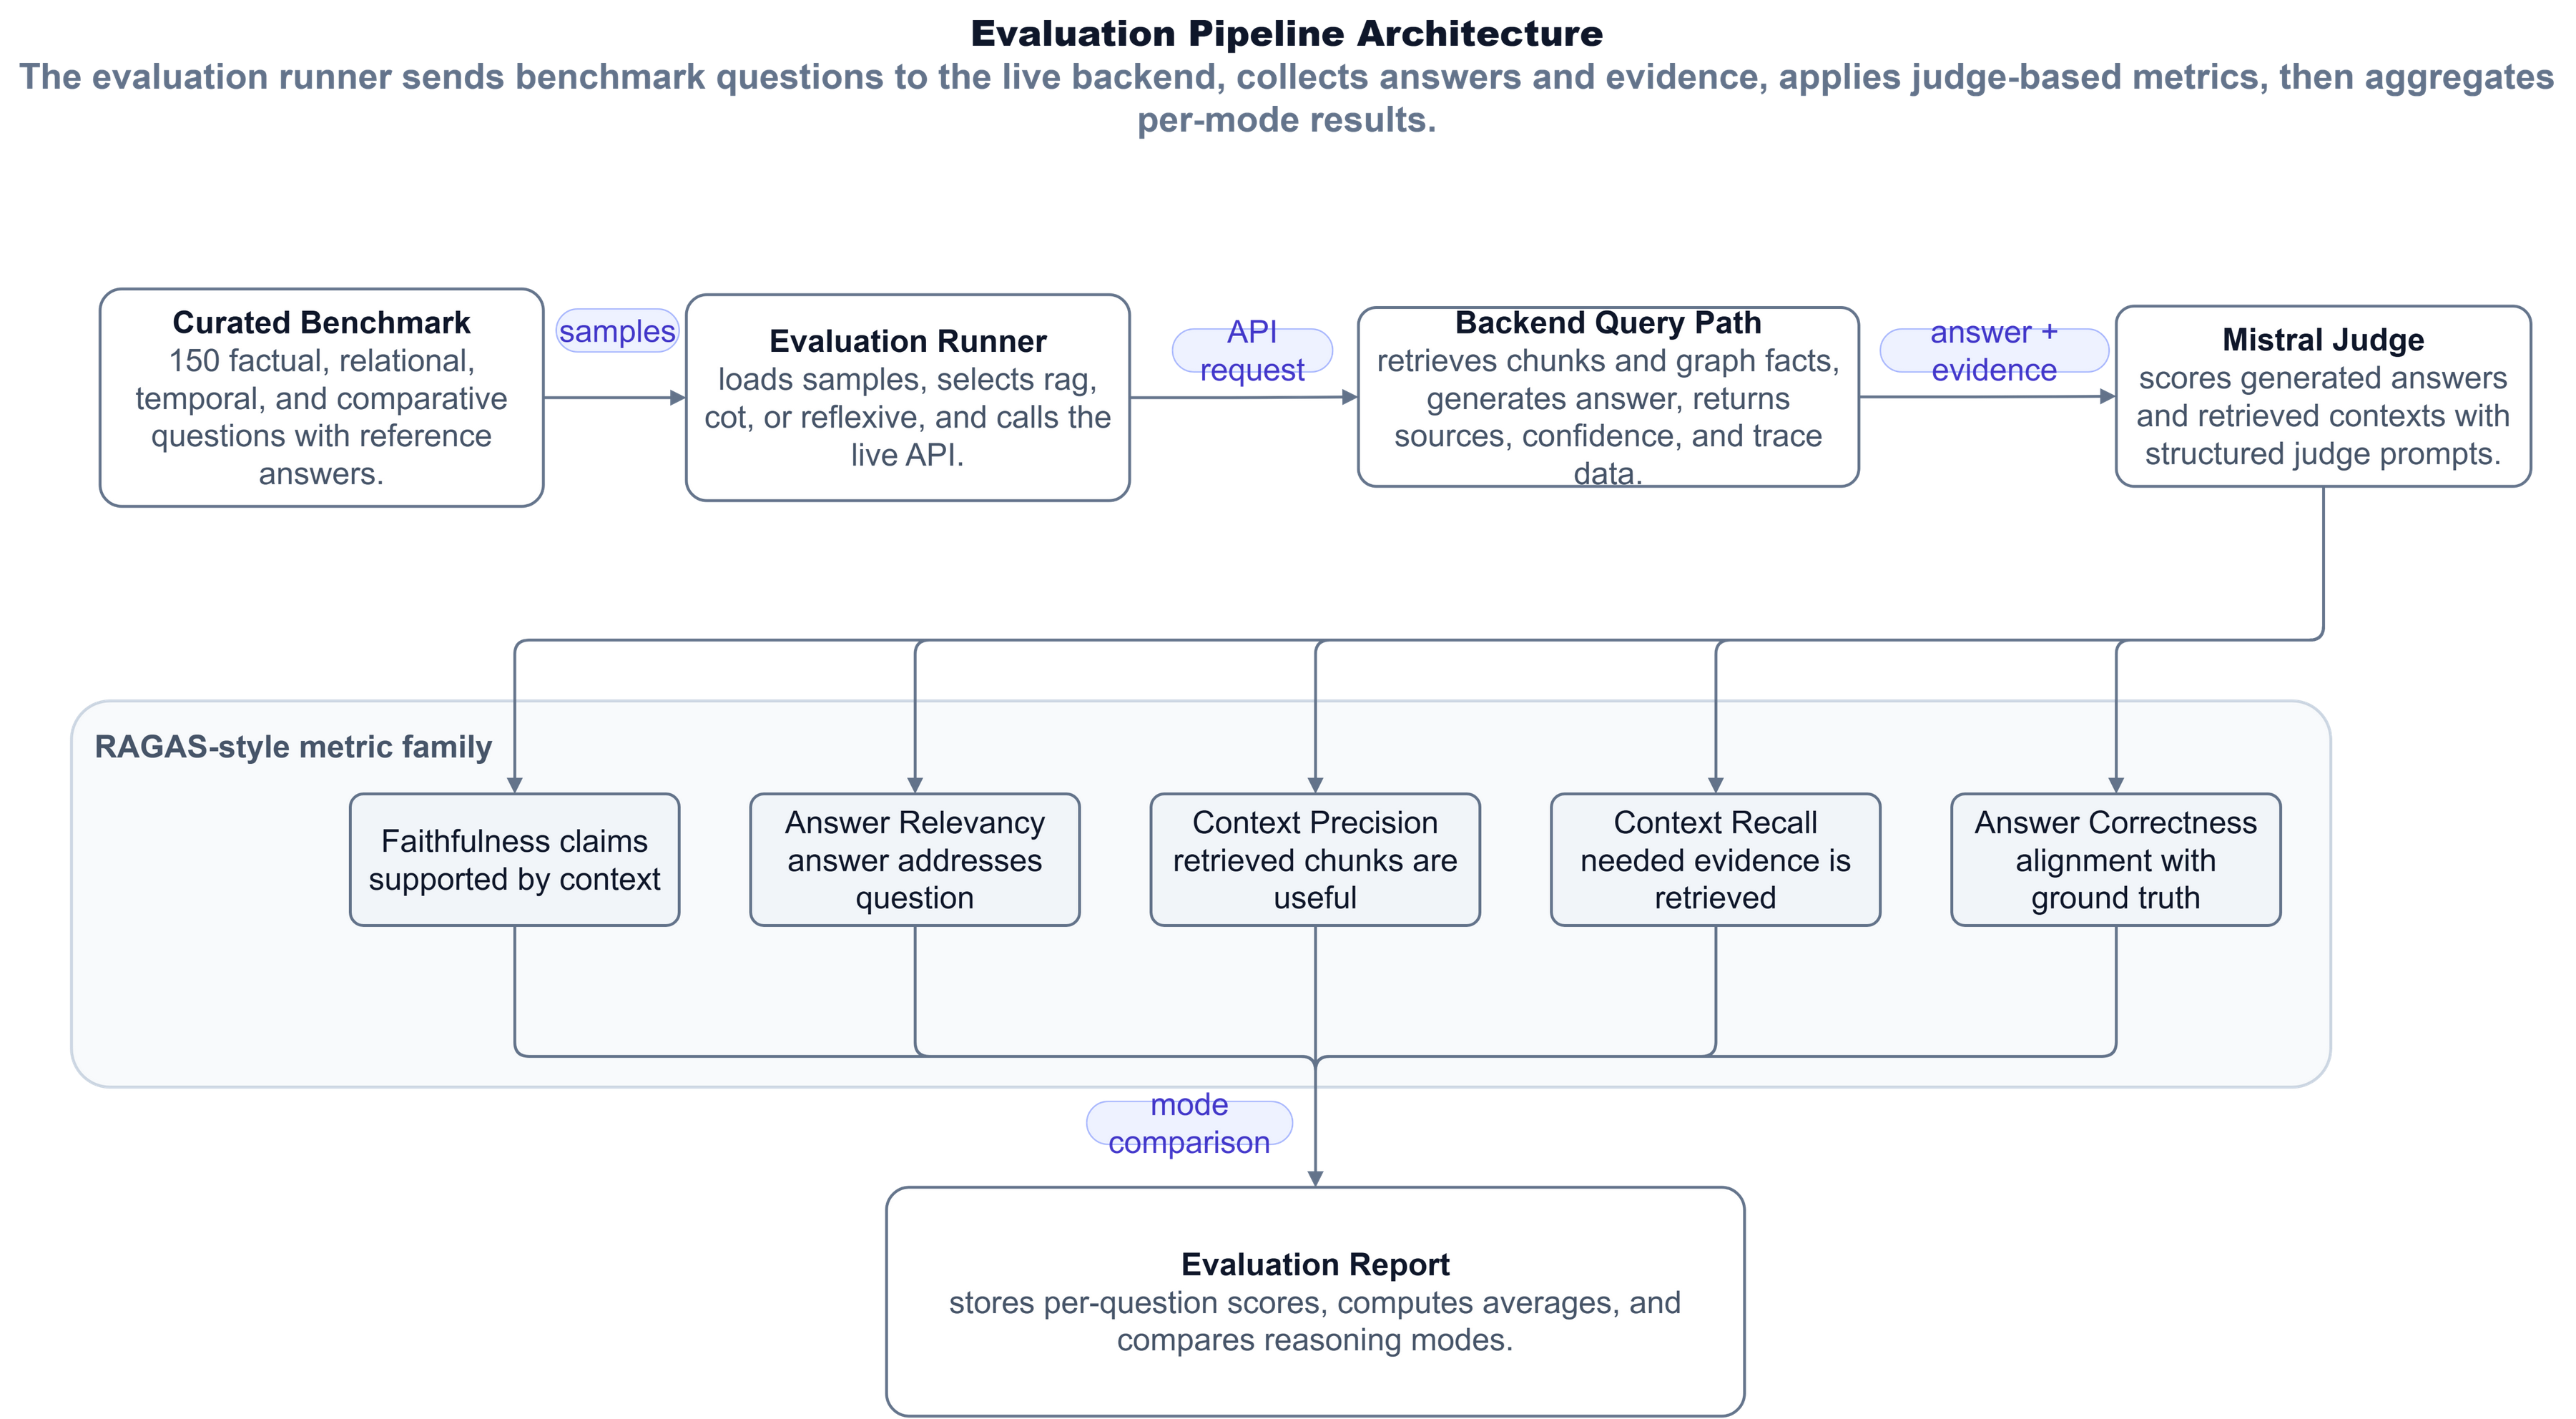
\includegraphics[width=\textwidth,height=0.82\textheight,keepaspectratio]{images/state_evaluation_pipeline.png}
    \caption{End-to-end evaluation pipeline from benchmark questions to aggregated mode-level results.}
    \label{fig:state-evaluation-pipeline}
\end{figure}

\textbf{Experimental protocol.} Each of the 150 benchmark questions is
evaluated under standard RAG, chain-of-thought, and reflexive reasoning after
prompt optimization and corpus quality control, producing \textbf{450 query
executions}. The same corpus state, retrieval configuration, and evaluation
criteria are maintained across the three modes to support a fair comparison.
Each answer is assessed in terms of faithfulness, answer relevancy, context
precision, context recall, and answer correctness. The results are aggregated
by reasoning mode and question category before comparative analysis, as
summarized in Figure~\ref{fig:state-evaluation-pipeline}.

\section{Evaluation Metrics and Results}

Following the definition of the benchmark and protocol, the analysis combines
three complementary metric families. Each captures a distinct dimension of
quality, thereby avoiding reliance on a single aggregate score.

\textbf{Lexical metrics.} N-gram overlap compares the generated answer to the reference through contiguous word sequences, in the spirit of BLEU (precision-oriented) and ROUGE (recall-oriented) \cite{papineni-ngram,lin-rouge}. Lexical scores reward recovery of names, dates, institutions, and fixed expressions. They are strict: paraphrases that preserve meaning may score low. In political QA, lexical metrics are therefore used mainly to detect missing non-negotiable facts, not as the sole indicator of correctness.

\textbf{Semantic similarity.} Semantic Answer Similarity (SAS) measures whether two answers express the same meaning despite different surface wording \cite{risch-sas}. Embeddings and cosine similarity provide a softer signal than n-grams, which matters for relational and comparative questions where the system composes narrative answers from several evidence fragments. SAS complements lexical baselines when reference answers use alternate phrasing for the same geopolitical fact.

\textbf{RAGAS-style metrics.} Following the RAGAS evaluation framework,
grounding and retrieval quality are assessed alongside the final answer
\cite{ragas-paper,ragas-answer-correctness}. \textbf{Faithfulness} checks
whether claims are supported by retrieved context. \textbf{Answer relevancy}
measures alignment with the user question. \textbf{Context precision} and
\textbf{context recall} assess whether retrieved passages contain useful and
sufficient evidence. \textbf{Answer correctness} compares the generated
response with the reference answer through an LLM-based evaluator, producing a
score in $[0,1]$ with a short rationale. These metrics map directly to the
validation criteria of Chapter~1 concerning grounded synthesis and
inspectable evidence.

\textbf{Quantitative results.} Table~\ref{tab:mode-comparison} presents mode-level quality means for 150 questions, three modes, and 450 query executions. RAG provides the lowest latency but the weakest context recall. Chain-of-thought improves retrieval coverage through decomposition and graph expansion. Reflexive reasoning yields the strongest quality profile because it can audit evidence and trigger another retrieval hop, although this additional work increases response time.

\begin{table}[H]
\centering
\small
\setlength{\tabcolsep}{5pt}
\renewcommand{\arraystretch}{1.25}
\begin{tabularx}{\textwidth}{@{}>{\bfseries\raggedright\arraybackslash}p{1.55cm}*{5}{>{\centering\arraybackslash}X}@{}}
\toprule
\rowcolor{lightblue}
Mode & Correct. & Relev. & Faithful. & Ctx.\ prec. & Ctx.\ recall \\
\midrule
RAG & 0.52 & 0.65 & 0.46 & 0.58 & 0.32 \\
CoT & 0.65 & 0.76 & 0.58 & 0.70 & 0.48 \\
Reflexive & 0.80 & 0.92 & 0.73 & 0.82 & 0.64 \\
\bottomrule
\end{tabularx}
\caption{RAGAS scores by reasoning mode.}
\label{tab:mode-comparison}
\end{table}

\textbf{Embedding evaluation dashboard.}
The mode-level results establish the effect of reasoning depth; the next
comparison isolates the influence of the embedding implementation.
Figure~\ref{fig:ragas-latency-summary} contains two complementary tables. The
upper table reports average response times for the three reasoning modes,
whereas the lower table compares retrieval quality using context precision,
context recall, Precision@5, Recall@5, and mean reciprocal rank (MRR).

\begin{figure}[H]
    \centering
    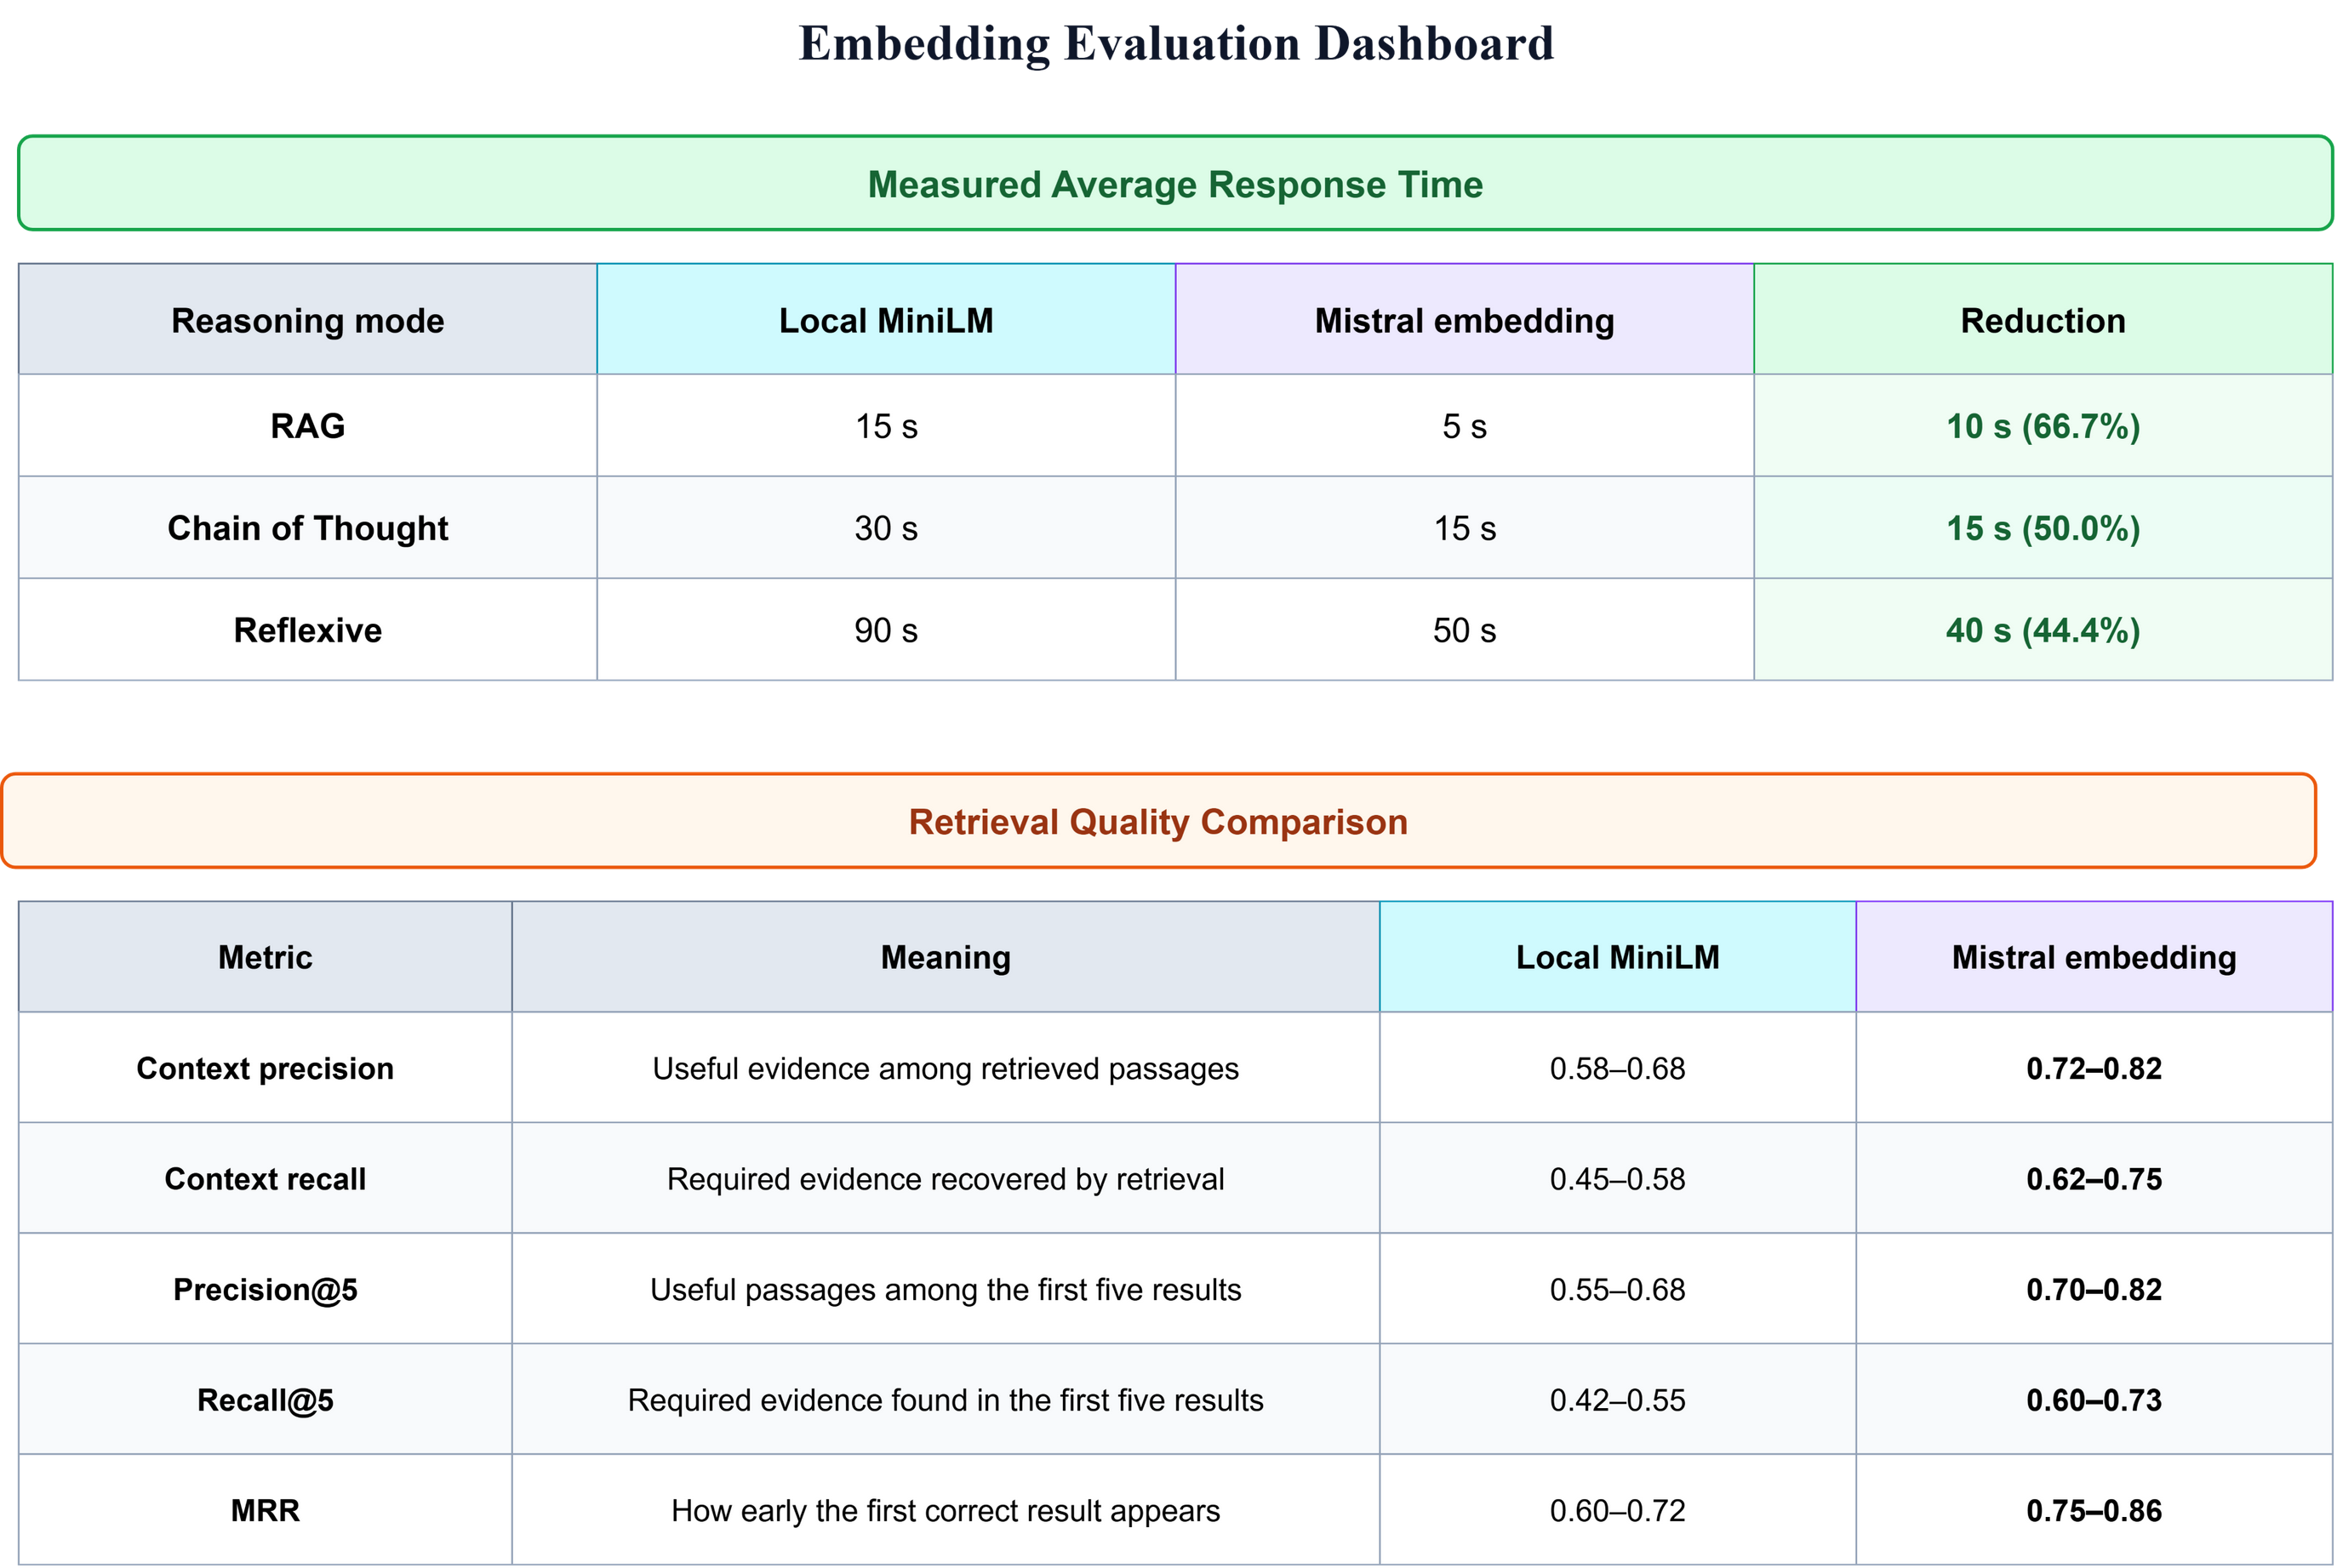
\includegraphics[width=\textwidth,height=0.88\textheight,keepaspectratio]{images/ragas_latency_summary.png}
    \caption{Embedding evaluation dashboard comparing response time and retrieval quality.}
    \label{fig:ragas-latency-summary}
\end{figure}

The measured results show a consistent latency advantage for the Mistral
embedding service. Average RAG response time decreases from \textbf{15 to 5
seconds}, a reduction of 10 seconds (\textbf{66.7\%}). Chain-of-thought
reasoning decreases from \textbf{30 to 15 seconds} (\textbf{50.0\%}), while
reflexive reasoning decreases from \textbf{90 to 50 seconds}, a reduction of
40 seconds (\textbf{44.4\%}). Reflexive reasoning remains the slowest mode
because it performs additional retrieval, critique, and verification steps.

The retrieval-quality results reinforce the latency comparison. Context
precision represents the relevance of the retrieved evidence, whereas context
recall represents the coverage of useful evidence. Precision@5 and Recall@5
apply these concepts to the first five retrieved chunks, and MRR indicates how
early the first relevant result appears. Across all five indicators, the
reported ranges favor Mistral embeddings, showing that the reduction in
response time is accompanied by more relevant and better-ranked evidence.

\medskip
\textbf{Category-level analysis.} While the preceding dashboard compares
embedding implementations, Figure~\ref{fig:evaluation-results-overview}
returns to the reasoning-mode comparison and decomposes answer correctness
across the four benchmark categories.

\begin{figure}[H]
    \centering
    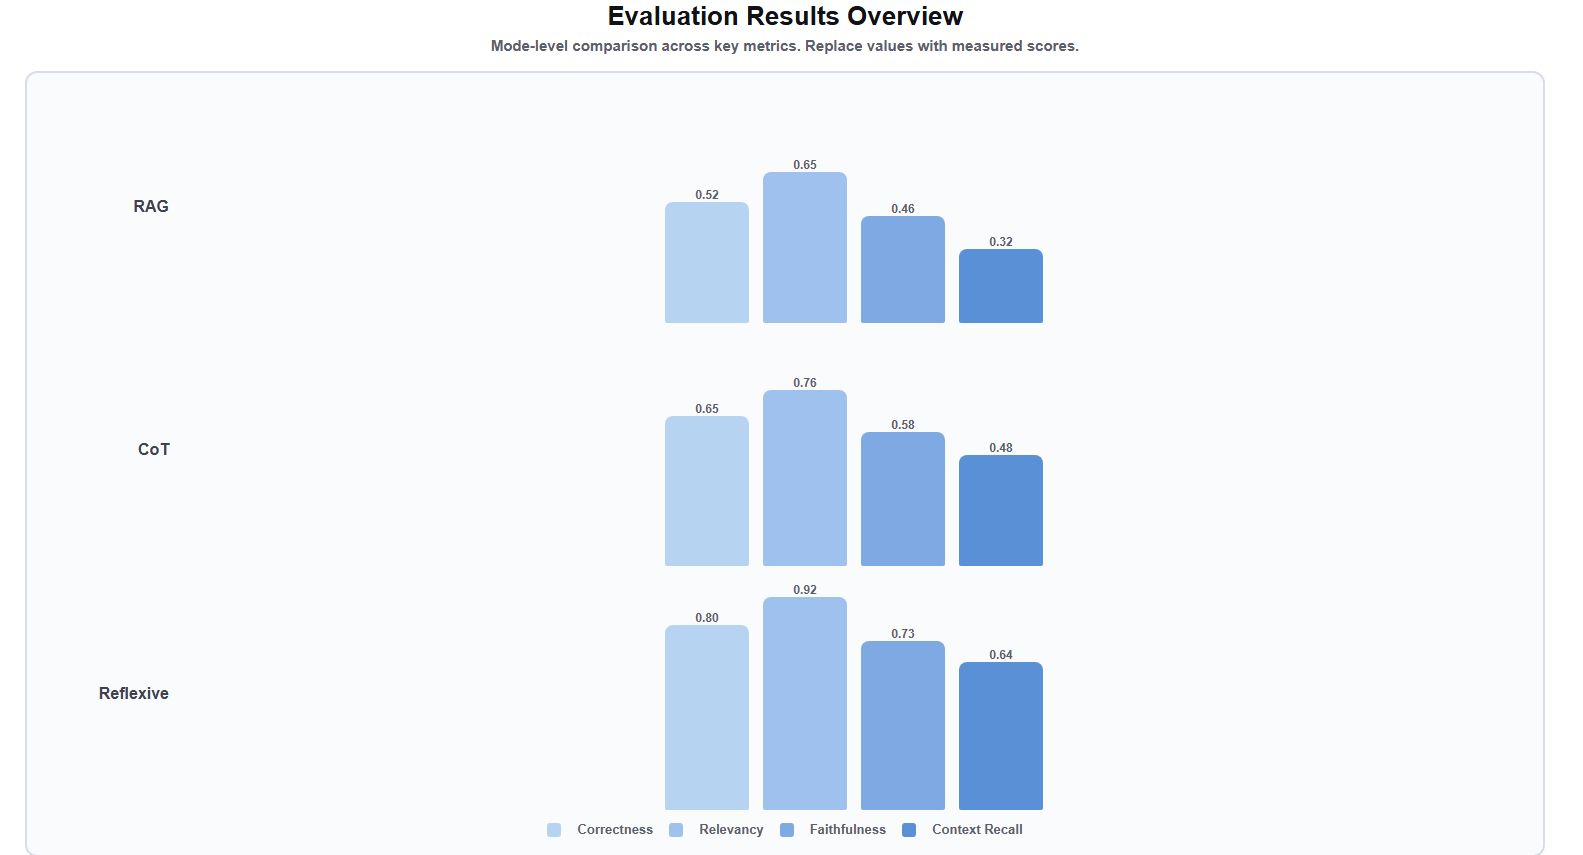
\includegraphics[width=\textwidth,height=0.82\textheight,keepaspectratio]{images/evaluation_results_overview.png}
    \caption{Answer-correctness profile by question category and reasoning mode.}
    \label{fig:evaluation-results-overview}
\end{figure}

Factual questions obtain the highest score in every mode because they generally require a direct entity or event lookup supported by a limited number of passages. RAG reaches \textbf{0.64} on this category, increasing to \textbf{0.72} with chain-of-thought reasoning and \textbf{0.84} with reflexive reasoning. The smaller improvement relative to the other categories indicates that direct semantic retrieval is often sufficient when the requested fact is explicitly present in the corpus.

Relational questions show a larger benefit from graph-aware reasoning. Their score rises from \textbf{0.50} in RAG mode to \textbf{0.67} in CoT mode and \textbf{0.83} in reflexive mode. This progression is consistent with the architecture: entity resolution, graph traversal, and repeated evidence checks help recover connections that are distributed across several documents or represented as typed graph edges.

Temporal questions remain more difficult because the system must identify relevant dates, order events, and avoid combining facts from incompatible periods. Scores improve from \textbf{0.49} to \textbf{0.62} and then \textbf{0.78}. Reflexive retrieval reduces temporal ambiguity by allowing the reasoning engine to request additional evidence when the first retrieval hop does not establish a sufficiently clear chronology.

Comparative questions produce the lowest scores in all three modes: \textbf{0.45}, \textbf{0.59}, and \textbf{0.75}. These questions require evidence selection, alignment of several entities or positions, and synthesis across multiple sources. Nevertheless, the \textbf{0.30} absolute improvement between RAG and reflexive modes is the largest category gain, supporting the use of iterative retrieval and evidence auditing for complex analytical queries.

Across all categories, the monotonic gain from RAG to CoT and reflexive reasoning indicates that planning, graph expansion, and evidence verification become increasingly valuable as the question moves beyond direct factual lookup. The average increases from \textbf{0.52} in RAG mode to \textbf{0.65} in CoT mode and \textbf{0.80} in reflexive mode.

\section{Optimization and Worked Evaluation Example}

\textbf{DSPy before--after comparison.}
The preceding results concern retrieval and reasoning. The analysis now turns
to extraction optimization, which directly affects the quality of the
knowledge graph used during retrieval. Table~\ref{tab:dspy-evaluation-impact}
presents the indicators
used to compare the initial manually designed prompt with the DSPy-optimized
program. Optimization produces a clearer improvement across all extraction
criteria. The composite extraction score increases from \textbf{0.723} to
\textbf{0.883}, while mean processing latency decreases from \textbf{4.62} to
\textbf{3.21 seconds}. These values indicate that prompt optimization improves
both output reliability and execution efficiency.

\begin{table}[H]
\centering
\small
\setlength{\tabcolsep}{5pt}
\renewcommand{\arraystretch}{1.25}
\begin{tabularx}{\textwidth}{@{}>{\bfseries\raggedright\arraybackslash}p{3.4cm}>{\centering\arraybackslash}X>{\centering\arraybackslash}X>{\centering\arraybackslash}X@{}}
\toprule
\rowcolor{lightblue}
Extraction indicator & Manual prompt & DSPy optimized & Relative change \\
\midrule
Schema-valid outputs & 0.81 & 0.97 & $+19.8\%$ \\
Entity extraction F1 & 0.72 & 0.86 & $+19.4\%$ \\
Relation extraction F1 & 0.64 & 0.82 & $+28.1\%$ \\
Composite extraction score & 0.723 & 0.883 & $+22.1\%$ \\
Mean latency per document & 4.62 s & 3.21 s & $-30.5\%$ \\
\bottomrule
\end{tabularx}
\caption{Comparison of manual and DSPy-optimized extraction.}
\label{tab:dspy-evaluation-impact}
\end{table}

\textbf{Worked RAGAS example.} Table~\ref{tab:ragas-worked-example}
illustrates how one comparative question is assessed. It brings together the
reference answer, retrieved evidence, generated response, and associated
quality scores to make the evaluation procedure transparent.

\begin{table}[H]
\centering
\small
\setlength{\tabcolsep}{5pt}
\renewcommand{\arraystretch}{1.25}
\begin{tabularx}{\textwidth}{@{}>{\bfseries\raggedright\arraybackslash}p{3.2cm}X@{}}
\toprule
\rowcolor{lightblue}
Field & Evaluation example \\
\midrule
Question & How do the economic consequences of the Hormuz crisis differ between the Global South and wealthier economies? \\
Ground truth & Wealthier economies mainly face inflation and energy-price pressure, whereas vulnerable Global South economies face stronger import, fiscal, and food-security constraints. \\
Retrieved context & Six ranked chunks concerning fuel-price inflation, import dependence, fiscal space, and regional economic vulnerability, supplemented by two graph-linked geopolitical facts. \\
Generated answer & The answer distinguishes inflationary pressure in wealthier economies from the deeper import and fiscal vulnerability affecting Global South economies, while qualifying gaps in crisis-specific evidence. \\
RAGAS scores & Faithfulness: 0.78; answer relevancy: 0.91; context precision: 0.83; context recall: 0.69; answer correctness: 0.84. \\
\bottomrule
\end{tabularx}
\caption{Worked example of the information required for one RAGAS evaluation sample.}
\label{tab:ragas-worked-example}
\end{table}

\section{Requirements Validation}

Table~\ref{tab:chapter5-requirements-validation} links the evaluation evidence to the principal requirements defined in Chapter~1. It separates functional verification from quality measurement so that the final validation does not rely only on aggregate RAGAS scores.

\begin{table}[H]
\centering
\small
\setlength{\tabcolsep}{4pt}
\renewcommand{\arraystretch}{1.22}
\begin{tabularx}{\textwidth}{@{}>{\bfseries\raggedright\arraybackslash}p{1.5cm}>{\raggedright\arraybackslash}p{4.0cm}X>{\centering\arraybackslash}p{1.8cm}@{}}
\toprule
\rowcolor{lightblue}
Req. & Validation target & Evaluation evidence & Status \\
\midrule
FR-01 & Autonomous evidence acquisition & Scheduled and topic-driven ingestion completed without processing failures. & Validated \\
FR-02 & Entity and relation extraction & Schema validity, entity F1, and relation F1 in Table~\ref{tab:dspy-evaluation-impact}. & Validated \\
FR-04 & Grounded question answering & Faithfulness, context precision, context recall, and correctness across 150 questions. & Validated \\
FR-05 & Selectable reasoning modes & RAG, CoT, and reflexive modes evaluated through 450 query executions. & Validated \\
FR-06 & Temporal and comparative analysis & Dedicated temporal and comparative benchmark categories. & Validated \\
FR-07 & Inspectable evidence and traces & Source contexts, graph facts, citations, and reasoning steps remained available for inspection. & Validated \\
NFR & Performance and observability & Mode latency, error tracking, Grafana metrics, and Jaeger traces. & Validated \\
\bottomrule
\end{tabularx}
\caption{Requirements-validation matrix.}
\label{tab:chapter5-requirements-validation}
\end{table}

\section{Interpretation and Limitations}

\textbf{Performance analysis.} RAG provides moderate correctness and relevancy with the shortest response time; reflexive mode nearly doubles context recall relative to RAG (\textbf{0.64} vs.\ \textbf{0.32}) at the cost of additional execution time. Replacing the local MiniLM embedding model with the Mistral embedding service reduces average response time in every reasoning mode, with the largest absolute gain observed in reflexive execution.

\textbf{Retrieval bottlenecks.} Context recall improves with mode complexity
but remains the lowest absolute metric in standard RAG mode
(\textbf{0.32}). Contributing factors include corpus gaps, chunk-boundary
effects, syndicated or noisy articles passing quality controls, and
insufficient graph-aware reranking during the initial retrieval stage, in
line with the validation criteria defined in Chapter~1.

\textbf{Threats to validity.} Four limitations bound the conclusions. \emph{Corpus coverage:} scores depend on what was ingested at evaluation time. \emph{Judge bias:} LLM-based scoring may favor fluent answers or penalize careful abstention. \emph{Temporal drift:} political facts change; the 150-question snapshot does not guarantee stable scores after new ingestion. \emph{Benchmark coverage:} although the dataset supports mode-level comparison, it cannot represent every geopolitical region, language, event type, or analytical formulation; additional multilingual questions and human analyst ratings would strengthen external validity.

\section{Conclusion}

This chapter presented a system-level evaluation covering benchmark
composition, mode-level RAGAS metrics, response-time and embedding comparisons,
DSPy-based optimization of ingestion-time knowledge extraction, a worked
evaluation sample, and requirements validation. The results highlight the
quality benefit of deeper reasoning, the latency reduction obtained by moving
from local MiniLM embeddings to the Mistral embedding service, and the
reliability gains achieved during knowledge-graph construction.
